\chapter{Signal-to-Noise Ratio (SNR)}
\label{ch:snr}

\begin{nontechnical}
\textbf{SNR is like trying to have a conversation}---in a quiet library (high SNR) you hear every word clearly, but in a loud nightclub (low SNR) you can barely understand anything!

\textbf{Simple idea:}
\begin{itemize}
\item \textbf{Signal} = the information you want (voice, data, music)
\item \textbf{Noise} = random interference you don't want (static, hiss)
\item \textbf{SNR} = how much stronger the signal is than the noise
\end{itemize}

\textbf{Real examples:}
\begin{itemize}
\item WiFi near router: 60~dB SNR $\rightarrow$ fast speeds (1~Gbps+)
\item WiFi far away: 10~dB SNR $\rightarrow$ slow speeds (10~Mbps)
\item Cell phone bars directly show SNR: 5 bars = high SNR, 1 bar = low SNR
\end{itemize}

\textbf{Why it matters:} Higher SNR means faster data rates, fewer errors, and better quality. Engineers constantly battle to maximize SNR in every communication system.
\end{nontechnical}

\section{Overview}

\textbf{Signal-to-Noise Ratio (SNR)} is a fundamental metric quantifying the quality of a received signal by comparing the power of the desired signal to the power of background noise. It directly determines system performance, including bit error rate (BER), achievable data rate, and link reliability.

\begin{keyconcept}
SNR is the \textbf{single most important parameter} in determining communication system performance. A 3~dB improvement in SNR can double the data rate or reduce BER by an order of magnitude. Every design decision in wireless systems---from antenna size to transmit power---ultimately targets SNR optimization.
\end{keyconcept}

SNR relates directly to Shannon's channel capacity theorem and sets fundamental limits on achievable data rates in the presence of noise.

\section{Mathematical Description}

\subsection{SNR Definition}

The Signal-to-Noise Ratio is defined as the ratio of signal power to noise power:
\begin{equation}
\mathrm{SNR} = \frac{P_s}{P_n}
\end{equation}
where:
\begin{itemize}
\item $P_s$ = signal power (watts)
\item $P_n$ = noise power (watts)
\end{itemize}

\subsection{Logarithmic (Decibel) Form}

In practice, SNR is expressed in decibels (dB):
\begin{equation}
\mathrm{SNR_{dB}} = 10\log_{10}\left(\frac{P_s}{P_n}\right)
\end{equation}

\textbf{Why decibels?} The logarithmic scale:
\begin{itemize}
\item Compresses enormous dynamic ranges (noise can be $10^{12}$ times weaker than signal)
\item Allows addition/subtraction instead of multiplication/division in link budgets
\item Aligns with human perception of signal quality
\end{itemize}

\begin{calloutbox}{Decibel Conversion Rules}
Useful approximations for quick calculations:
\begin{itemize}
\item $+3$~dB $\approx$ double the power (exactly $2\times$)
\item $+10$~dB $=$ exactly $10\times$ the power
\item $+20$~dB $=$ exactly $100\times$ the power
\item $0$~dB $=$ equal signal and noise power
\item Negative dB $=$ noise stronger than signal
\end{itemize}
\end{calloutbox}

\subsection{Voltage-Based SNR}

When measuring voltage instead of power:
\begin{equation}
\mathrm{SNR_{dB}} = 20\log_{10}\left(\frac{V_s}{V_n}\right)
\end{equation}
where:
\begin{itemize}
\item $V_s$ = signal RMS voltage
\item $V_n$ = noise RMS voltage
\end{itemize}

Note the factor of 20 instead of 10, since $P \propto V^2$.

\subsection{Energy Ratios}

For digital communications, SNR relates to energy-per-bit:
\begin{equation}
\frac{E_b}{N_0} = \mathrm{SNR} \cdot \frac{B}{R_b}
\end{equation}
where:
\begin{itemize}
\item $E_b$ = energy per bit (joules)
\item $N_0$ = noise power spectral density (W/Hz)
\item $B$ = bandwidth (Hz)
\item $R_b$ = bit rate (bps)
\end{itemize}

\subsection{Carrier-to-Noise Ratio (CNR)}

In RF systems, often measured as Carrier-to-Noise Ratio:
\begin{equation}
\mathrm{CNR} = \frac{P_c}{P_n} = \frac{A_c^2 / 2}{N_0 B}
\end{equation}
where:
\begin{itemize}
\item $P_c$ = carrier power (watts)
\item $A_c$ = carrier amplitude
\item $N_0$ = noise power spectral density (W/Hz)
\item $B$ = receiver bandwidth (Hz)
\end{itemize}

For unmodulated carriers, CNR $=$ SNR.

\section{SNR Visualization}

\subsection{SNR Concept Diagram}

SNR quantifies the separation between desired signal and unwanted noise:

\begin{center}
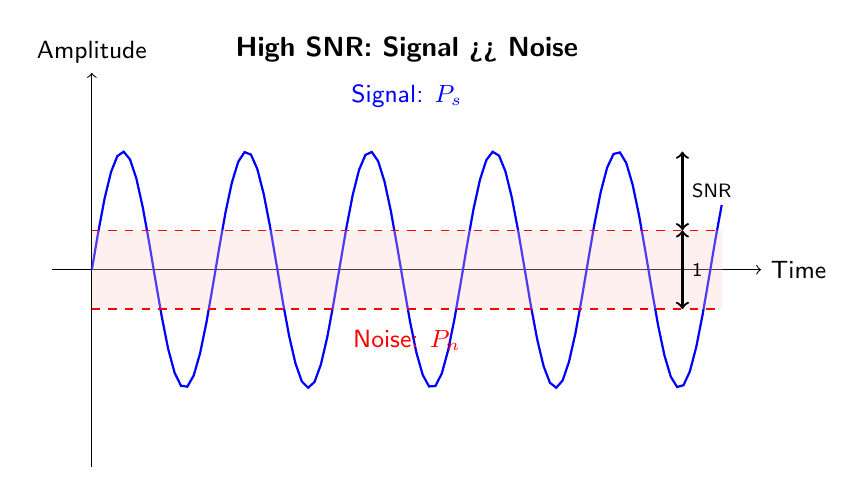
\begin{tikzpicture}[scale=1.0]
% Axes
\draw[->] (-0.5,0) -- (8.5,0) node[right,font=\sffamily\small] {Time};
\draw[->] (0,-2.5) -- (0,2.5) node[above,font=\sffamily\small] {Amplitude};

% Clean signal
\draw[thick,blue] plot[domain=0:8,samples=100] (\x,{1.5*sin(4*\x r)});
\node[blue,font=\sffamily\small] at (4,2.2) {Signal: $P_s$};

% Noise floor
\fill[red!20,opacity=0.3] (0,-0.5) rectangle (8,0.5);
\draw[red,dashed] (0,0.5) -- (8,0.5);
\draw[red,dashed] (0,-0.5) -- (8,-0.5);
\node[red,font=\sffamily\small] at (4,-0.9) {Noise: $P_n$};

% SNR annotation
\draw[<->,thick,black] (7.5,0.5) -- (7.5,1.5);
\node[right,font=\sffamily\scriptsize] at (7.5,1.0) {SNR};
\draw[<->,thick,black] (7.5,-0.5) -- (7.5,0.5);
\node[right,font=\sffamily\scriptsize] at (7.5,0) {1};

% Title
\node[font=\sffamily\bfseries] at (4,2.8) {High SNR: Signal >> Noise};
\end{tikzpicture}
\end{center}

\begin{center}
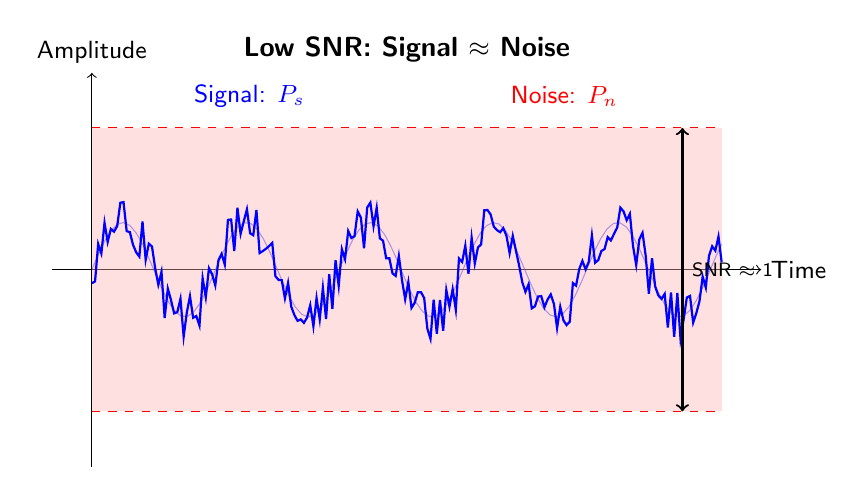
\begin{tikzpicture}[scale=1.0]
% Axes
\draw[->] (-0.5,0) -- (8.5,0) node[right,font=\sffamily\small] {Time};
\draw[->] (0,-2.5) -- (0,2.5) node[above,font=\sffamily\small] {Amplitude};

% Signal with heavy noise
\draw[blue,opacity=0.5] plot[domain=0:8,samples=100] (\x,{0.6*sin(4*\x r)});

% Heavy noise
\fill[red!30,opacity=0.4] (0,-1.8) rectangle (8,1.8);
\draw[red,dashed] (0,1.8) -- (8,1.8);
\draw[red,dashed] (0,-1.8) -- (8,-1.8);

% Noisy signal overlay
\draw[thick,blue] plot[domain=0:8,samples=200] (\x,{0.6*sin(4*\x r) + 0.3*rand});
\node[blue,font=\sffamily\small] at (2,2.2) {Signal: $P_s$};
\node[red,font=\sffamily\small] at (6,2.2) {Noise: $P_n$};

% SNR annotation
\draw[<->,thick,black] (7.5,-1.8) -- (7.5,1.8);
\node[right,font=\sffamily\scriptsize] at (7.5,0) {SNR $\approx$ 1};

% Title
\node[font=\sffamily\bfseries] at (4,2.8) {Low SNR: Signal $\approx$ Noise};
\end{tikzpicture}
\end{center}

\subsection{SNR Measurement Setup}

\begin{center}
\begin{tikzpicture}[
  block/.style={rectangle, draw, minimum width=2.5cm, minimum height=1cm, font=\sffamily\small},
  node distance=2.5cm,
  font=\small
]
% Transmitter
\node[block] (tx) {Transmitter\\$P_t$};

% Channel
\node[block, right of=tx, minimum width=3cm] (channel) {Channel\\+ Noise};
\node[below=0.3cm of channel, font=\scriptsize] {AWGN: $N_0$};

% Receiver
\node[block, right of=channel] (rx) {Receiver\\$P_r$};

% Power meter
\node[block, below=1.5cm of rx] (meter) {Power\\Meter};

% Arrows
\draw[->,thick] (tx) -- node[above,font=\scriptsize] {$P_s$} (channel);
\draw[->,thick] (channel) -- node[above,font=\scriptsize] {$P_s + P_n$} (rx);
\draw[->,thick] (rx) -- (meter);

% Measurement annotation
\node[below=0.1cm of meter, align=center, font=\scriptsize] {
  Measure: $P_s$ (signal on)\\
  Measure: $P_n$ (signal off)\\
  Compute: SNR $= P_s/P_n$
};

% Antenna symbols
\draw[thick] (tx.east) ++(0.8,0.3) -- ++(0.3,0.3) -- ++(-0.3,0.3);
\draw[thick] (tx.east) ++(0.8,-0.3) -- ++(0.3,-0.3) -- ++(-0.3,-0.3);
\draw[thick] (channel.west) ++(-0.8,0.3) -- ++(-0.3,0.3) -- ++(0.3,0.3);
\draw[thick] (channel.west) ++(-0.8,-0.3) -- ++(-0.3,-0.3) -- ++(0.3,-0.3);
\end{tikzpicture}
\end{center}

\subsection{SNR Impact on Constellation}

\begin{center}
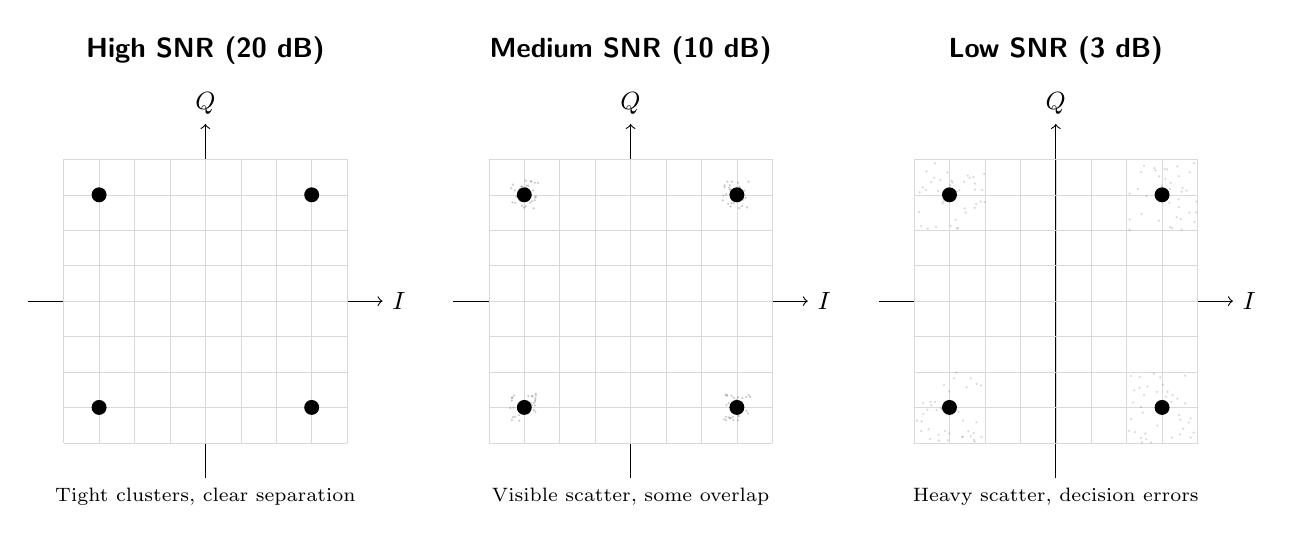
\begin{tikzpicture}[scale=0.9]
% High SNR constellation
\begin{scope}[shift={(0,0)}]
\node[above,font=\sffamily\bfseries] at (0,3.2) {High SNR (20 dB)};
\draw[->] (-2.5,0) -- (2.5,0) node[right,font=\sffamily\small] {$I$};
\draw[->] (0,-2.5) -- (0,2.5) node[above,font=\sffamily\small] {$Q$};
\draw[very thin,gray!30] (-2,-2) grid[step=0.5] (2,2);

% QPSK constellation with tight clusters
\foreach \x/\y in {-1.5/1.5, 1.5/1.5, -1.5/-1.5, 1.5/-1.5} {
  \fill[black] (\x,\y) circle (3pt);
  \foreach \i in {1,...,20} {
    \fill[black,opacity=0.3] (\x+0.05*rand,\y+0.05*rand) circle (0.5pt);
  }
}
\node[below,font=\scriptsize] at (0,-2.5) {Tight clusters, clear separation};
\end{scope}

% Medium SNR constellation
\begin{scope}[shift={(6,0)}]
\node[above,font=\sffamily\bfseries] at (0,3.2) {Medium SNR (10 dB)};
\draw[->] (-2.5,0) -- (2.5,0) node[right,font=\sffamily\small] {$I$};
\draw[->] (0,-2.5) -- (0,2.5) node[above,font=\sffamily\small] {$Q$};
\draw[very thin,gray!30] (-2,-2) grid[step=0.5] (2,2);

% QPSK constellation with moderate scatter
\foreach \x/\y in {-1.5/1.5, 1.5/1.5, -1.5/-1.5, 1.5/-1.5} {
  \fill[black] (\x,\y) circle (3pt);
  \foreach \i in {1,...,30} {
    \fill[black,opacity=0.2] (\x+0.2*rand,\y+0.2*rand) circle (0.5pt);
  }
}
\node[below,font=\scriptsize] at (0,-2.5) {Visible scatter, some overlap};
\end{scope}

% Low SNR constellation
\begin{scope}[shift={(12,0)}]
\node[above,font=\sffamily\bfseries] at (0,3.2) {Low SNR (3 dB)};
\draw[->] (-2.5,0) -- (2.5,0) node[right,font=\sffamily\small] {$I$};
\draw[->] (0,-2.5) -- (0,2.5) node[above,font=\sffamily\small] {$Q$};
\draw[very thin,gray!30] (-2,-2) grid[step=0.5] (2,2);

% QPSK constellation with heavy scatter
\foreach \x/\y in {-1.5/1.5, 1.5/1.5, -1.5/-1.5, 1.5/-1.5} {
  \fill[black] (\x,\y) circle (3pt);
  \foreach \i in {1,...,40} {
    \fill[black,opacity=0.15] (\x+0.5*rand,\y+0.5*rand) circle (0.5pt);
  }
}
\node[below,font=\scriptsize] at (0,-2.5) {Heavy scatter, decision errors};
\end{scope}
\end{tikzpicture}
\end{center}

\subsection{SNR in Chimera}\label{snr-in-chimera}

In Chimera\textquotesingle s simulation, you control the \textbf{channel
SNR}, which determines how much noise is added to the transmitted
signal:

{\def\LTcaptype{} % do not increment counter
\begin{longtable}[]{@{}lll@{}}
\toprule\noalign{}
Setting & Description & Constellation \\
\midrule\noalign{}
\endhead
\bottomrule\noalign{}
\endlastfoot
\textbf{High SNR} (-5 dB) & Minimal noise & Tight clusters \\
\textbf{Medium SNR} (-15 dB) & Moderate noise & Visible scatter \\
\textbf{Low SNR} (-25 dB) & Heavy noise & Large scatter, errors
likely \\
\end{longtable}
}

\subsubsection{Processing Gain}\label{processing-gain}

Chimera achieves approximately \textbf{35 dB of processing gain} through
symbol averaging and oversampling. This means:

\begin{verbatim}
Effective SNR = Channel SNR + Processing Gain
              = -25 dB + 35 dB
              = 10 dB (after processing)
\end{verbatim}

This is why the system can operate reliably even with very low channel
SNR values.

\subsection{SNR vs $E_s/N_0$ and $E_b/N_0$}

Different SNR definitions are used depending on context:

\begin{equation}
\mathrm{SNR} = \frac{P_s}{P_n} = \frac{E_s / T_s}{N_0 / T_s} = \frac{E_s}{N_0}
\end{equation}
where:
\begin{itemize}
\item $E_s$ = energy per symbol (joules)
\item $T_s$ = symbol duration (seconds)
\end{itemize}

Relationship to $E_b/N_0$:
\begin{equation}
\frac{E_b}{N_0} = \frac{E_s}{N_0 \cdot \log_2(M)} = \frac{\mathrm{SNR}}{\log_2(M)}
\end{equation}
where $M$ is the modulation order (e.g., $M=2$ for BPSK, $M=4$ for QPSK).

\begin{warningbox}
Be careful when comparing SNR values: specify whether it's $E_b/N_0$, $E_s/N_0$, or carrier SNR. For QPSK: $E_b/N_0 = E_s/N_0 - 3$~dB since each symbol carries 2 bits.
\end{warningbox}

\section{SNR and Bit Error Rate (BER)}

\subsection{Theoretical BER for BPSK}

In AWGN channels, BER depends directly on SNR:
\begin{equation}
\mathrm{BER} = Q\left(\sqrt{\frac{2E_b}{N_0}}\right) = Q\left(\sqrt{2 \cdot \mathrm{SNR}}\right)
\end{equation}
where $Q(x)$ is the Gaussian Q-function:
\begin{equation}
Q(x) = \frac{1}{\sqrt{2\pi}} \int_x^\infty e^{-t^2/2}\,dt
\end{equation}

\subsection{Key SNR Thresholds}

\textbf{For BPSK in AWGN:}
\begin{itemize}
\item $E_b/N_0 = 4$~dB: BER $\approx 10^{-2}$ (1 error per 100 bits)
\item $E_b/N_0 = 7$~dB: BER $\approx 10^{-3}$ (1 error per 1,000 bits)
\item $E_b/N_0 = 9.6$~dB: BER $\approx 10^{-5}$ (1 error per 100,000 bits)
\item $E_b/N_0 = 11$~dB: BER $\approx 10^{-6}$ (1 error per million bits)
\end{itemize}

\textbf{Rule of thumb:} Increasing $E_b/N_0$ by 2~dB reduces BER by approximately one order of magnitude in the region around $10^{-3}$ to $10^{-6}$.

\subsection{Impact of SNR on Performance}

\begin{center}
\begin{tabular}{clll}
\toprule
\textbf{SNR (dB)} & \textbf{Quality} & \textbf{BER} & \textbf{Impact} \\
\midrule
$>20$ & Excellent & $<10^{-6}$ & Near-perfect reception \\
$10-20$ & Good & $10^{-3}$ to $10^{-6}$ & Reliable with FEC \\
$5-10$ & Fair & $10^{-2}$ to $10^{-3}$ & Heavy FEC required \\
$0-5$ & Poor & $>10^{-2}$ & High error rate \\
$<0$ & Very Poor & $>10^{-1}$ & Marginal or unusable \\
\bottomrule
\end{tabular}
\end{center}

\section{Shannon's Channel Capacity}

The fundamental relationship between SNR and maximum achievable data rate is given by Shannon's theorem:
\begin{equation}
C = B \log_2(1 + \mathrm{SNR})
\end{equation}
where:
\begin{itemize}
\item $C$ = channel capacity (bps)
\item $B$ = bandwidth (Hz)
\item SNR = linear signal-to-noise ratio (not in dB)
\end{itemize}

\subsection{Practical Implications}

Converting to decibels:
\begin{equation}
C = B \log_2\left(1 + 10^{\mathrm{SNR_{dB}}/10}\right)
\end{equation}

\textbf{Key insights:}
\begin{itemize}
\item Doubling SNR increases capacity by less than 1 bit/s/Hz
\item At high SNR: each 3~dB increase adds $\sim$0.5 bits/s/Hz
\item At low SNR: capacity increases nearly linearly with SNR
\item No coding scheme can exceed this fundamental limit
\end{itemize}

\begin{calloutbox}{Spectral Efficiency vs SNR}
Modern systems operate near Shannon capacity:
\begin{itemize}
\item WiFi 6 (1024-QAM): requires 35~dB SNR for 10 bits/s/Hz
\item LTE (64-QAM): requires 18~dB SNR for 5 bits/s/Hz
\item Satellite (QPSK): requires 10~dB SNR for 2 bits/s/Hz
\item Shannon limit for 30~dB SNR: $\log_2(1001) \approx 10$ bits/s/Hz
\end{itemize}
\end{calloutbox}

\section{Noise Sources and SNR Degradation}

\subsection{Thermal Noise}

The fundamental noise floor in all receivers:
\begin{equation}
P_n = kTB
\end{equation}
where:
\begin{itemize}
\item $k = 1.38 \times 10^{-23}$~J/K (Boltzmann constant)
\item $T$ = system noise temperature (K)
\item $B$ = bandwidth (Hz)
\end{itemize}

In decibels:
\begin{equation}
P_n = -174 + 10\log_{10}(B) + 10\log_{10}\left(\frac{T}{290}\right) \text{ dBm}
\end{equation}

At room temperature ($T = 290$~K):
\begin{equation}
P_n = -174 + 10\log_{10}(B) \text{ dBm/Hz}
\end{equation}

\subsection{Noise Figure}

Real receivers add noise beyond thermal noise:
\begin{equation}
F = \frac{\mathrm{SNR_{in}}}{\mathrm{SNR_{out}}}
\end{equation}
where:
\begin{itemize}
\item $F$ = noise figure (linear ratio)
\item $\mathrm{SNR_{in}}$ = SNR at receiver input
\item $\mathrm{SNR_{out}}$ = SNR at receiver output
\end{itemize}

In decibels:
\begin{equation}
NF = 10\log_{10}(F) = \mathrm{SNR_{in,dB}} - \mathrm{SNR_{out,dB}}
\end{equation}

Effective noise power:
\begin{equation}
N_{\mathrm{eff}} = kTBF = N_{\mathrm{thermal}} \cdot F
\end{equation}

\section{Worked Example: Satellite Downlink SNR}

\textbf{Scenario:} Calculate received SNR for a geostationary satellite TV downlink

\subsection*{Given Parameters}

\begin{tabular}{@{}ll@{}}
Satellite TX power & $P_t = 100$~W = 50~dBm \\
TX antenna gain & $G_t = 32$~dBi \\
Distance (GEO orbit) & $d = 36{,}000$~km \\
Frequency & $f = 12$~GHz (Ku-band) \\
RX dish diameter & $D = 0.6$~m \\
RX antenna gain & $G_r = 37$~dBi \\
System noise temp & $T_s = 200$~K \\
Bandwidth & $B = 36$~MHz \\
\end{tabular}

\subsection*{Required}

Find the received SNR.

\subsection*{Solution}

\textit{Step 1: Calculate Free-Space Path Loss (FSPL)}

\begin{equation}
\mathrm{FSPL} = 20\log_{10}(d) + 20\log_{10}(f) + 32.45
\end{equation}
\begin{equation}
\mathrm{FSPL} = 20\log_{10}(36{,}000{,}000) + 20\log_{10}(12{,}000) + 32.45
\end{equation}
\begin{equation}
\mathrm{FSPL} = 151.1 + 81.6 + 32.45 = 205.2~\text{dB}
\end{equation}

\textit{Step 2: Calculate Received Signal Power}

\begin{equation}
P_r = P_t + G_t + G_r - \mathrm{FSPL}
\end{equation}
\begin{equation}
P_r = 50 + 32 + 37 - 205.2 = -86.2~\text{dBm}
\end{equation}

\textit{Step 3: Calculate Noise Power}

\begin{equation}
N = kT_sB = (1.38 \times 10^{-23})(200)(36 \times 10^6)
\end{equation}
\begin{equation}
N = 9.94 \times 10^{-14}~\text{W} = -100.0~\text{dBm}
\end{equation}

\textit{Step 4: Calculate SNR}

\begin{equation}
\mathrm{SNR} = P_r - N = -86.2 - (-100.0) = 13.8~\text{dB}
\end{equation}

\subsection*{Answer}

The received SNR is \textbf{13.8~dB}.

\subsection*{Interpretation}

This SNR is sufficient for reliable QPSK reception with forward error correction (FEC). Typical satellite systems require 10--15~dB SNR for acceptable TV quality. Higher-order modulation (8PSK, 16-APSK) would require additional SNR margin.

\section{Applications}

\subsection{Wireless Communication Systems}

\subsubsection{WiFi (802.11ax)}

\begin{itemize}
\item \textbf{Adaptive modulation:} Automatically selects modulation order based on SNR
\item \textbf{1024-QAM mode:} Requires SNR $>35$~dB for 10--12~Gbps
\item \textbf{BPSK fallback:} Used at SNR $<5$~dB for reliability at 6--9~Mbps
\item \textbf{Link adaptation:} Measures SNR every 100~ms and adjusts rate
\end{itemize}

\subsubsection{LTE/5G Cellular}

\begin{itemize}
\item \textbf{SINR (Signal-to-Interference-plus-Noise-Ratio):} Extends SNR concept for multi-cell interference
\item \textbf{CQI (Channel Quality Indicator):} Reports SNR to base station every 5~ms
\item \textbf{MCS (Modulation and Coding Scheme):} 29 combinations from QPSK+FEC to 256-QAM+light FEC
\item \textbf{Typical SINR:} 0--5~dB at cell edge, 15--25~dB near base station
\end{itemize}

\subsection{Satellite Communications}

\subsubsection{DVB-S2X (Satellite TV)}

\begin{itemize}
\item \textbf{VCM (Variable Coding and Modulation):} Adapts to rain fade
\item \textbf{SNR range:} $-2$~dB (QPSK) to $+16$~dB (32-APSK)
\item \textbf{Rain margin:} Typical link designed with 3--6~dB excess SNR
\item \textbf{Adaptive coding:} LDPC codes rated from 1/4 to 9/10
\end{itemize}

\subsubsection{Deep Space Network}

\begin{itemize}
\item \textbf{Operating SNR:} Typically $-5$ to $+5$~dB (negative SNR common!)
\item \textbf{Giant antennas:} 70~m dishes provide 74~dBi gain
\item \textbf{Turbo codes:} Within 1~dB of Shannon limit
\item \textbf{Example:} Voyager 1 operates at effective SNR near 0~dB
\end{itemize}

\subsection{Audio and Video Systems}

\subsubsection{Professional Audio}

\begin{itemize}
\item \textbf{Studio standard:} SNR $>90$~dB (A-weighted)
\item \textbf{CD quality:} 96~dB theoretical (16-bit quantization)
\item \textbf{Consumer electronics:} 60--80~dB typical
\item \textbf{Measurement:} Referenced to maximum undistorted signal level
\end{itemize}

\section{Improving SNR: Practical Techniques}

\subsection{Increase Signal Power}

\begin{equation}
\mathrm{SNR_{new}} = \mathrm{SNR_{old}} + \Delta P_t
\end{equation}

\textbf{Methods:}
\begin{itemize}
\item Increase transmit power (limited by regulations and power consumption)
\item Use higher-gain antennas ($G_t$ or $G_r$ increase)
\item Reduce path loss (shorter distance, higher frequency efficiency)
\end{itemize}

\subsection{Reduce Noise Power}

\begin{equation}
\mathrm{SNR_{new}} = \mathrm{SNR_{old}} - \Delta N
\end{equation}

\textbf{Methods:}
\begin{itemize}
\item Reduce receiver bandwidth (if signal bandwidth permits)
\item Lower noise figure (better LNA design)
\item Cool receiver (cryogenic for satellite ground stations)
\item Improve shielding (reduce external interference)
\end{itemize}

\subsection{Processing Gain}

For spread spectrum systems:
\begin{equation}
G_p = \frac{B_{\mathrm{spread}}}{B_{\mathrm{signal}}}
\end{equation}
where:
\begin{itemize}
\item $G_p$ = processing gain
\item $B_{\mathrm{spread}}$ = spreading bandwidth
\item $B_{\mathrm{signal}}$ = information bandwidth
\end{itemize}

Effective SNR improvement:
\begin{equation}
\mathrm{SNR_{effective}} = \mathrm{SNR_{channel}} + 10\log_{10}(G_p)
\end{equation}

\textbf{Examples:}
\begin{itemize}
\item GPS L1 C/A: 43~dB processing gain (1.023~MHz / 50~Hz)
\item CDMA cellular: 21~dB processing gain (1.25~MHz / 9.6~kHz)
\item LoRa IoT: 20--30~dB processing gain
\end{itemize}

\section{Summary}

\begin{center}
\begin{tabular}{ll}
\toprule
\textbf{Parameter} & \textbf{Description} \\
\midrule
Definition & Ratio of signal power to noise power \\
Units & Linear (ratio) or dB (logarithmic) \\
Formula & $\mathrm{SNR_{dB}} = 10\log_{10}(P_s/P_n)$ \\
Typical range & $-10$~dB (deep space) to $+60$~dB (WiFi) \\
Shannon limit & $C = B\log_2(1 + \mathrm{SNR})$ \\
BER relationship & Exponential: 2~dB $\approx$ 10$\times$ BER reduction \\
Noise floor & $-174$~dBm/Hz at 290~K \\
\bottomrule
\end{tabular}
\end{center}

\subsection*{Key Points}

\begin{itemize}
\item SNR fundamentally determines system performance (BER, capacity, range)
\item 3~dB improvement doubles effective signal power
\item Shannon capacity sets theoretical limit: $C = B\log_2(1 + \mathrm{SNR})$
\item Thermal noise floor: $-174$~dBm/Hz limits all systems
\item Modern systems operate 1--3~dB from Shannon limit
\end{itemize}

\subsection*{Advantages of High SNR}

\begin{itemize}
\item Higher-order modulation possible (greater spectral efficiency)
\item Lower bit error rates (fewer retransmissions)
\item Simplified receiver design (less sophisticated equalization)
\item Reduced forward error correction overhead
\end{itemize}

\subsection*{Design Trade-offs}

\begin{itemize}
\item Power vs battery life (mobile devices)
\item Antenna size vs portability
\item Bandwidth vs noise power
\item Cost vs noise figure performance
\end{itemize}

\section{Further Reading}

\begin{itemize}
\item For energy ratio definitions: Chapter~\ref{ch:energy-ratios}
\item For noise fundamentals: Chapter~\ref{ch:awgn}
\item For BER analysis: Chapter~\ref{ch:ber}
\item For Shannon's theorem: Chapter~\ref{ch:shannon}
\item For link budget analysis: Chapter~\ref{ch:link-budget}
\item For constellation effects: Chapter~\ref{ch:constellation}
\end{itemize}
